%\title{EMC LaTeX Portrait Poster Template}
%%%%%%%%%%%%%%%%%%%%%%%%%%%%%%%%%%%%%%%%%
% a1poster Portrait Poster
% LaTeX Template
% Version 2.0 (22/06/16)
%
% The a1poster class was created by:
% Joe Rowing (JoeRowing@exeterms.ac.uk)
% 
% This template has been produced by:
% Joe Rowing at Exeter Mathematics School
%
% License:
% CC BY-NC-SA 3.0 (http://creativecommons.org/licenses/by-nc-sa/3.0/)
%
%%%%%%%%%%%%%%%%%%%%%%%%%%%%%%%%%%%%%%%%%

%----------------------------------------------------------------------------------------
%   PACKAGES AND OTHER DOCUMENT CONFIGURATIONS
%----------------------------------------------------------------------------------------

\documentclass[a1,portrait]{a1poster}

\usepackage{multicol} % This is so we can have multiple columns of text side-by-side
\columnsep=50pt % This is the amount of white space between the columns in the poster
\columnseprule=0.01pt % This is the thickness of the black line between the columns in the poster

\usepackage[svgnames]{xcolor} % Specify colors by their 'svgnames', for a full list of all colors available see here: http://www.latextemplates.com/svgnames-colors

\usepackage{times} % Use the times font


\usepackage{graphicx} % Required for including images
\graphicspath{{figures/}} % Location of the graphics files
\usepackage{booktabs} % Top and bottom rules for table
\usepackage[font=small,labelfont=bf]{caption} % Required for specifying captions to tables and figures
\usepackage{amsfonts, amsmath, amsthm, amssymb} % For math fonts, symbols and environments
\usepackage{wrapfig} % Allows wrapping text around tables and figures

\begin{document}

%----------------------------------------------------------------------------------------
%   POSTER HEADER 
% The header is divided into two boxes:
% The first is 75% wide and houses the title, subtitle, names, university/organization and contact information
% The second is 25% wide and houses the EMS Logo
% 
%----------------------------------------------------------------------------------------

\begin{minipage}[b]{0.6\linewidth}
\huge \color{DarkRed} \textbf{Quick and Reusable Code Generation for Idris} \color{Black}\\ % Title
\huge\textit{Integrating dependent types into the industrial services}\\[1cm] % Subtitle
\large \textbf{Taine Zhao \& Yukiyoshi Kameyama}\\[0.5cm] % Author(s)
\large Computer Science, University of Tsukuba \\[0.2cm] % University/organization
\texttt{thaut@logic.cs.tsukuba.ac.jp; kam@cs.tsukuba.ac.jp}\\
\end{minipage}
%
% \begin{minipage}[b]{0.4\linewidth}
% 
\includegraphics[width=15cm]{emsnew.PNG}\\
% \end{minipage}

\vspace{.5cm} % A bit of extra whitespace between the header and poster content

%----------------------------------------------------------------------------------------

\begin{multicols}{2} % This is how many columns your poster will be broken into, by convention a portrait poster is generally split into 2 or 3 columns

%----------------------------------------------------------------------------------------
%   ABSTRACT

%An abstract is a brief summary of a research article, thesis, review, conference proceeding or any in-depth analysis of a particular subject and is often used to help the reader quickly ascertain the paper's purpose
%----------------------------------------------------------------------------------------

\color{CornflowerBlue} % Colour for the abstract

\section*{Abstract}

As a dependently-typed functional programming languages, Idris shows
quite a high expressiveness with its type system under a considerably strong static guarantee.

To leverage these powerful static programming language features for
existing industrial applications safer and more expressive,
we're supposed to implement code generation back ends for Idris.

Whereas Idris has already provided convenient interfaces to support
agnostic back ends, it is still cumbersome to import Idris programs
into an existing programming language, as the latter is already
in a large amount and continuously proliferating, and the implementations
of each back end certainly have quite a few overlaps.
  
To address this, we introduce a "common" intermediate representation
powered by Tagless Final Style, which contributes to the reuse most of the tasks
required by an Idris back end. As a result, we allow making a Idris back end
in a most simplified routine, which can usually be accomplished in few hours
or even minutes.

%----------------------------------------------------------------------------------------
%   INTRODUCTION

%Avoid using technical definitions unless absolutely necessary. The introduction section is here to introduce your issue, so be sure to not bore your readers right away with excessive information. You can even include graphics if they will help the viewer understand the work that you have done.
%----------------------------------------------------------------------------------------

\color{Red} % color for the introduction

\section*{Introduction}

Aliquam non lacus dolor, \textit{a aliquam quam} \cite{Smith:2012qr}. Cum sociis natoque penatibus et magnis dis parturient montes, nascetur ridiculus mus. Nulla in nibh mauris. Donec vel ligula nisi, a lacinia arcu. Sed mi dui, malesuada vel consectetur et, egestas porta nisi. Sed eleifend pharetra dolor, et dapibus est vulputate eu. \textbf{Integer faucibus elementum felis vitae fringilla.} In hac habitasse platea dictumst. Duis tristique rutrum nisl, nec vulputate elit porta ut. Donec sodales sollicitudin turpis sed convallis. Etiam mauris ligula, blandit adipiscing condimentum eu, dapibus pellentesque risus.

\textit{Aliquam auctor}, metus id ultrices porta, risus enim cursus sapien, quis iaculis sapien tortor sed odio. Mauris ante orci, euismod vitae tincidunt eu, porta ut neque. Aenean sapien est, viverra vel lacinia nec, venenatis eu nulla. Maecenas ut nunc nibh, et tempus libero. Aenean vitae risus ante. Pellentesque condimentum dui. Etiam sagittis purus non tellus tempor volutpat. Donec et dui non massa tristique adipiscing.

%----------------------------------------------------------------------------------------
%   OBJECTIVES
%----------------------------------------------------------------------------------------

\color{Black} % DarkSlateGray color for the rest of the content

\section*{Main Objectives}

\begin{enumerate}
\item Lorem ipsum dolor sit amet, consectetur.
\item Nullam at mi nisl. Vestibulum est purus, ultricies cursus volutpat sit amet, vestibulum eu.
\item Praesent tortor libero, vulputate quis elementum a, iaculis.
\item Phasellus a quam mauris, non varius mauris. Fusce tristique, enim tempor varius porta, elit purus commodo velit, pretium mattis ligula nisl nec ante.
\item Ut adipiscing accumsan sapien, sit amet pretium.
\item Estibulum est purus, ultricies cursus volutpat
\item Nullam at mi nisl. Vestibulum est purus, ultricies cursus volutpat sit amet, vestibulum eu.
\item Praesent tortor libero, vulputate quis elementum a, iaculis.
\end{enumerate}

%----------------------------------------------------------------------------------------
%   MATERIALS AND METHODS

% In this section you will cover the materials and methods (shocking!) that you used in your research process. Feel free to include any images, charts, or graphs here that will help the viewer better understand your process. Also, don’t forget to provide a rationale to explain why you chose these methods! This is just as important as the steps you took
%----------------------------------------------------------------------------------------

\section*{Materials and Methods}

Fusce magna risus, molestie ut porttitor in, consectetur sed mi. Vestibulum ante ipsum primis in faucibus orci luctus et ultrices posuere cubilia Curae; Pellentesque consectetur blandit pellentesque. Sed odio justo, viverra nec porttitor vel, lacinia a nunc. Suspendisse pulvinar euismod arcu, sit amet accumsan enim fermentum quis. In id mauris ut dui feugiat egestas. Vestibulum ac turpis lacinia nisl commodo sagittis eget sit amet sapien.

%------------------------------------------------

\subsection*{Mathematical Section}

Nulla vel nisl sed mauris auctor mollis non sed. 

\begin{equation}
E = mc^{2}
\label{eqn:Einstein}
\end{equation}

Curabitur mi sem, pulvinar quis aliquam rutrum. (1) edf (2)
, $\Omega=[-1,1]^3$, maecenas leo est, ornare at. $z=-1$ edf $z=1$ sed interdum felis dapibus sem. $x$ set $y$ ytruem. 
Turpis $j$ amet accumsan enim $y$-lacina; 
ref $k$-viverra nec porttitor $x$-lacina. 

Vestibulum ac diam a odio tempus congue. Vivamus id enim nisi:

\begin{eqnarray}
\cos\bar{\phi}_k Q_{j,k+1,t} + Q_{j,k+1,x}+\frac{\sin^2\bar{\phi}_k}{T\cos\bar{\phi}_k} Q_{j,k+1} &=&\nonumber\\ 
-\cos\phi_k Q_{j,k,t} + Q_{j,k,x}-\frac{\sin^2\phi_k}{T\cos\phi_k} Q_{j,k}\label{edgek}
\end{eqnarray}
and
\begin{eqnarray}
\cos\bar{\phi}_j Q_{j+1,k,t} + Q_{j+1,k,y}+\frac{\sin^2\bar{\phi}_j}{T\cos\bar{\phi}_j} Q_{j+1,k}&=&\nonumber \\
-\cos\phi_j Q_{j,k,t} + Q_{j,k,y}-\frac{\sin^2\phi_j}{T\cos\phi_j} Q_{j,k}.\label{edgej}
\end{eqnarray} 

Nulla sed arcu arcu. Duis et ante gravida orci venenatis tincidunt. Fusce vitae lacinia metus. Pellentesque habitant morbi. $\mathbf{A}\underline{\xi}=\underline{\beta}$ Vim $\underline{\xi}$ enum nidi $3(P+2)^{2}$ lacina. Id feugain $\mathbf{A}$ nun quis; magno.

%----------------------------------------------------------------------------------------
%   RESULTS 

%It’s always a good idea to begin the Results section with an initial summary of your results. Don’t address your research question just yet; instead, just address the general aspects of the data you collected or the number of valid data obtained.

%In your next paragraph, you can discuss the relationship between the data and your research question. What exactly does your data mean? Be sure to include any graphics that can help show you data visually, as the readers can understand graphics more easily and quickly than blocks of text.

%Sometimes less is more. Be selective when deciding what images, charts, and graphs make it onto your poster! 

%Charts and graphs are usually more effective than tables, but whatever you choose to use, make sure everything is labeled clearly! A graph with missing labels or a table without a title will just leave the reader confused. Also, carefully consider what type of chart or graph will best show your results. K. Broman, professor of Biostatistics & Medical Informatics at the University of Wisconsin Madison has written a great article titled, “The Top Ten Worst Graphs.” (http://www.biostat.wisc.edu/~kbroman/topten_worstgraphs/)
%----------------------------------------------------------------------------------------

\section*{Results}


Donec faucibus purus at tortor egestas eu fermentum dolor facilisis. Maecenas tempor dui eu neque fringilla rutrum. Mauris \emph{lobortis} nisl accumsan. Aenean vitae risus ante.
%
\begin{wraptable}{l}{12cm} % Left or right alignment is specified in the first bracket, the width of the table is in the second
\begin{tabular}{l l l}
\toprule
\textbf{Treatments} & \textbf{Response 1} & \textbf{Response 2}\\
\midrule
Treatment 1 & 0.0003262 & 0.562 \\
Treatment 2 & 0.0015681 & 0.910 \\
Treatment 3 & 0.0009271 & 0.296 \\
\bottomrule
\end{tabular}
\captionof{table}{\color{DarkRed} Table caption}
\end{wraptable}
%
Phasellus imperdiet, tortor vitae congue bibendum, felis enim sagittis lorem, et volutpat ante orci sagittis mi. Morbi rutrum laoreet semper. Morbi accumsan enim nec tortor consectetur non commodo nisi sollicitudin. Proin sollicitudin. Pellentesque eget orci eros. Fusce ultricies, tellus et pellentesque fringilla, ante massa luctus libero, quis tristique purus urna nec nibh.

Nulla ut porttitor enim. Suspendisse venenatis dui eget eros gravida tempor. Mauris feugiat elit et augue placerat ultrices. Morbi accumsan enim nec tortor consectetur non commodo. Pellentesque condimentum dui. Etiam sagittis purus non tellus tempor volutpat. Donec et dui non massa tristique adipiscing. Quisque vestibulum eros eu. Phasellus imperdiet, tortor vitae congue bibendum, felis enim sagittis lorem, et volutpat ante orci sagittis mi. Morbi rutrum laoreet semper. Morbi accumsan enim nec tortor consectetur non commodo nisi sollicitudin.

\begin{center}\vspace{1cm}
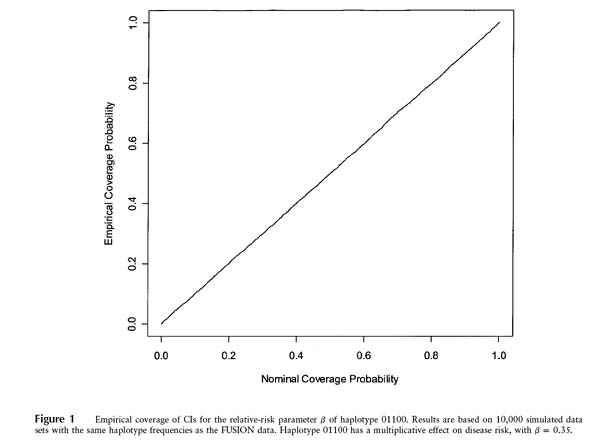
\includegraphics[width=0.5\linewidth]{epstein_fig1}
\captionof{figure}{\color{DarkRed} Figure caption}
\end{center}\vspace{1cm}

In hac habitasse platea dictumst. Etiam placerat, risus ac.

Adipiscing lectus in magna blandit:

\begin{center}\vspace{1cm}
\begin{tabular}{l l l l}
\toprule
\textbf{Treatments} & \textbf{Response 1} & \textbf{Response 2} \\
\midrule
Treatment 1 & 0.0003262 & 0.562 \\
Treatment 2 & 0.0015681 & 0.910 \\
Treatment 3 & 0.0009271 & 0.296 \\
\bottomrule
\end{tabular}
\captionof{table}{\color{DarkRed} Table caption}
\end{center}\vspace{1cm}

Vivamus sed nibh ac metus tristique tristique a vitae ante. Sed lobortis mi ut arcu fringilla et adipiscing ligula rutrum. Aenean turpis velit, placerat eget tincidunt nec, ornare in nisl. In placerat.

\begin{center}\vspace{1cm}
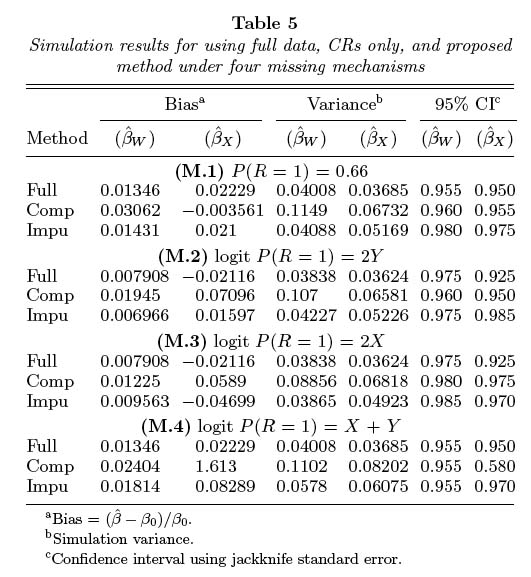
\includegraphics[width=0.5\linewidth]{paik_tab5}
\captionof{figure}{\color{DarkRed} Figure caption}
\end{center}\vspace{1cm}

%----------------------------------------------------------------------------------------
%   CONCLUSIONS
%In your conclusion section you want to briefly review your research questions and the results you obtain. You also should add why your results are interesting or significant. TIPS: Relate your results to other published research in the field. This will give your research more impact on your readers as well as show your professionalism in the study. You can also suggest continuing research that would build upon your current study.
%----------------------------------------------------------------------------------------

\color{FireBrick} %  colour for the conclusions to make them stand out

\section*{Conclusions}

\begin{itemize}
\item Pellentesque eget orci eros. Fusce ultricies, tellus et pellentesque fringilla, ante massa luctus libero, quis tristique purus urna nec nibh. Phasellus fermentum rutrum elementum. Nam quis justo lectus.
\item Vestibulum sem ante, hendrerit a gravida ac, blandit quis magna.
\item Donec sem metus, facilisis at condimentum eget, vehicula ut massa. Morbi consequat, diam sed convallis tincidunt, arcu nunc.
\item Nunc at convallis urna. isus ante. Pellentesque condimentum dui. Etiam sagittis purus non tellus tempor volutpat. Donec et dui non massa tristique adipiscing.
\end{itemize}

\color{Black} % Set the color back to DarkSlateGray for the rest of the content

%----------------------------------------------------------------------------------------
%   FORTHCOMING RESEARCH
%----------------------------------------------------------------------------------------

\section*{Forthcoming Research}

Vivamus molestie, risus tempor vehicula mattis, libero arcu volutpat purus, sed blandit sem nibh eget turpis. Maecenas rutrum dui blandit lorem vulputate gravida. Praesent venenatis mi vel lorem tempor at varius diam sagittis. Nam eu leo id turpis interdum luctus a sed augue. Nam tellus.

 %----------------------------------------------------------------------------------------
%   REFERENCES
%If you have an extremely extensive list of references, you may want to break it into 2 columns. 

% It is common to shrink the font of the References section if it becomes overbearing and long

%----------------------------------------------------------------------------------------
\begin{small}%Makes the text of the references section smaller
\begin{multicols}{2}%Makes the section two col
\nocite{*} % Print all references regardless of whether they were cited in the poster or not
\bibliographystyle{plain} % Plain referencing style
\bibliography{bibliography} % Use the example bibliography file sample.bib
\end{multicols}
\end{small}
%----------------------------------------------------------------------------------------
%   ACKNOWLEDGEMENTS
%You can acknowledge people who have helped you with your work, such as other members of your research group or your funding source. If there are any conflicts of interest regarding you and the work you have presented, be sure to include that here. It is always important to keep you and your work above reproach. Keep this section as short as possible. Fewer than 40 words is best.
%----------------------------------------------------------------------------------------

\section*{Acknowledgements}

Etiam fermentum, arcu ut gravida fringilla, dolor arcu laoreet justo, ut imperdiet urna arcu a arcu. Donec nec ante a dui tempus consectetur. Cras nisi turpis, dapibus sit amet mattis sed, laoreet.

%----------------------------------------------------------------------------------------
%	 CONTACT DETAILS
%A lot of posters include this section so the readers are able to contact the author later or read more about the research. You can include your email or website address, links to relevant resources, or even a QR code (What is a QR Code?) that viewers can scan to go directly to your website or a PDF version of your poster. If you choose to include this section, keep it very brief
%----------------------------------------------------------------------------------------
\section*{Contact Details}
Joe Rowing - JoeRowing@exeterms.ac.uk
\end{multicols}
\end{document}
